\documentclass[12pt]{exam}

\usepackage{amssymb}
\usepackage{mathtools}
\usepackage{algorithm}
\usepackage{float}  % Figure placement
\usepackage{minted}  % Code highlighting
\usepackage{tikz}  % Flow chart
\usepackage{lipsum}
\usepackage{xspace}
\usepackage{hyperref}
\usepackage{MnSymbol}
\usepackage{pgffor}
\usepackage{mdframed}



\hypersetup{
    colorlinks = true,
    linkcolor = blue,
    urlcolor  = blue,
    citecolor = blue,
    anchorcolor = blue
}

\newcommand{\hwheaderfooter}[3]{
\pagestyle{headandfoot}
\firstpageheadrule
\firstpageheader{#1}{#2}{#3}
\runningheader{#1}{#2}{#3}
\runningheadrule
\firstpagefooter{}{\thepage}{}
\runningfooter{}{\thepage}{}
}

\newcommand{\latex}{\LaTeX\xspace}

\newcommand{\stars}[1]{%
    \foreach \n in {1,...,#1}{%
        $\filledstar$%
    }%
}

\hwheaderfooter{HW 5}{Ching}{CSCI 406}


\begin{document}
\begin{center}
    \fbox{\fbox{\parbox{\textwidth - 0.2 in}{\centering

                {Instructions: Please note that handwritten assignments \textbf{will not be graded}. Use the
                    provided \latex template to complete your homework. Please do not alter the order or spacing of
                    questions (keep each question on its own page). When you submit to Gradescope, you must mark
                    which page(s) correspond to each question. \textbf{You may not receive credit for unmarked
                        questions}. \\ When including graphical figures, we encourage the use of tools such as \href{https://dreampuf.github.io/GraphvizOnline/}{graphviz} or packages like \href{https://www.overleaf.com/learn/latex/TikZ_package}{tikz} for simple and complex figures. However, these may be handwritten only if they are neat and legible (as defined by the grader). }\\

            }}}
\end{center}

\textbf{List any collaborators (besides TAs or professors) here:} N/A

\begin{questions}

    \question[30] [W6, \stars{5}] Graph Modelling. [{\bf Note: Similar to the maze project, this is a graph modeling question.}] Consider the following problem:

    \begin{mdframed}
        You are given a connected weighted graph $G$ that represents a road network connecting $n$ cities. An edge $(i,j)$ in $G$ means that there is a road segment from city $i$ to city $j$. The weight of edge $(i,j)$ denoted by $l_{ij}$ is the length of that road segment, which is {\em assumed to be an integer}. In addition, let $p_i$ denote the price of one unit of fuel at each city $i$ (assume that there are no gas stations on road segments and that fuel can only be purchased in cities). Finally, let $C$ (also an integer) denote the fuel tank capacity of your car. Determine the cheapest trip cost from start city $s$ to end city $e$. Your car uses one unit of fuel per unit of distance traveled and starts with an empty tank. You may choose to fill up your fuel tank by any integer amount as long as you don't exceed $C$.
    \end{mdframed}

    Describe a graph model (vertices and edges) that will enable one call of \textbf{unmodified} Dijkstra's to solve this problem. \textbf{Note:} we recommend that you define some notation to help you thoroughly describe your model.

    \begin{parts}
        \part[5] Describe what each vertex of your graph represents. (Hint: there will be at most $n \times (C+1)$ nodes in your model.)

        Each vertex represents a configuration of the car's fuel level $(0-C)$ and the city the car is in. That is, for every city $n$, there will be $C+1$ vertices representing the fuel level at that city. The vertex will be represented as $(k, f)$ where $k$ is the city and $f$ is the fuel level.

        \part[15] Describe the conditions necessary for an edge to exist between two vertices in your graph. (Hint: think about actions that might change the state of your model.)

        An edge exists between two vertices $(i,f)$ and $(j,g)$ if the the following conditions are met:
        \begin{itemize}
            \item There is a road segment between the two cities $i$ and $j$ in graph $G$.
            \item The fuel level $f$ is greater than or equal to the distance between the two cities $l_{ij}$.
            \item The fuel level $g=f-l_{ij}$.
            \item The fuel level $f$ is less than or equal to $C$ and the fuel level $g$ is greater than or equal to $0$. \textit{This should be taken care of by the node generation process.}
        \end{itemize}

        There will also be edges from $(i,f)$ and $(i,g)$ represented by the action of refueling at a city if the following conditions are met:
        \begin{itemize}
            \item Where the fuel level $g$ represents all integers greater than $f$.
            \item The fuel level $f$ and $g$ are less than or equal to $C$. \textit{This should be taken care of by the node generation process.}
        \end{itemize}

        \part[10] Describe how you would calculate the cost of an edge in your graph. Please provide a general mathematical expression (formula) for the edge weights. Note you might have different formulas for different edges, make sure to describe the conditions under which you would use each formula.

        The cost of an edge in the graph is the cost of the fuel used to travel from one city to another. The cost of the edge $(i,f)$ and $(j,g)$ is given by the formula:
        \[
            \text{cost} = 0
        \]
        this is because the cost of the fuel is occurs in the city $i$ not during transit.

        The cost of the edge $(i,f)$ and $(i,g)$ is given by the formula:
        \[
            \text{cost} = (g-f) \times p_i
        \]
        where $p_i$ is the price of fuel at city $i$ and $g-f$ is the amount of fuel used to refuel at city $i$.



    \end{parts}

    \clearpage

    \question[15] [W6, \stars{2}] Provide an example of a directed graph with a negative weight edge, and a specific start and end node such that a Dijkstra's search (that is, Dijkstra's algorithm with the modification that it terminates after the end node is deleted from the priority queue) will \textbf{not} give the correct answer. Your example shouldn't need more than a handful of vertices.

    \begin{figure}[H]
        \centering
        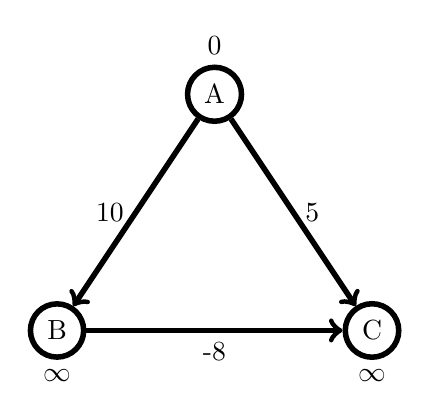
\begin{tikzpicture}
            % Nodes
            \node[circle, draw, line width=2pt] (A) at (0, 0) {A};
            \node[circle, draw, line width=2pt] (B) at (-2, -3) {B};
            \node[circle, draw, line width=2pt] (C) at (2, -3) {C};

            % Additional labels
            \node[above] at (A.north) {0};
            \node[below] at (B.south) {$\infty$};
            \node[below] at (C.south) {$\infty$};

            % Edges
            \draw[->, line width=2pt] (A) -- (B) node[midway, left] {10};
            \draw[->, line width=2pt] (A) -- (C) node[midway, right] {5};
            \draw[->, line width=2pt] (B) -- (C) node[midway, below] {-8};
        \end{tikzpicture}
        \caption{Example of a directed graph with a negative weight edge.}
        \label{fig:graph1}
    \end{figure}

    In the graph in Figure \ref{fig:graph1}, if we start at node A and end at node C, Dijkstra's algorithm will not give the correct answer. The algorithm will choose the path $A \rightarrow C$ with a total weight of 5, but the correct shortest path is $A \rightarrow B \rightarrow C$ with a total weight of 2.

    This is because after the first iteration of Dijkstra's algorithm, the algorithm will traverse to nodes $B$ and $C$ and set their distances to accordingly, as shown in Figure \ref{fig:Dijkstra}. Dijkstra's will then check the priority queue and find that the next node to visit is $C$. The algorithm will then terminate and return the shortest path to $C$ as the shortest path.

    \begin{figure}[H]
        \centering
        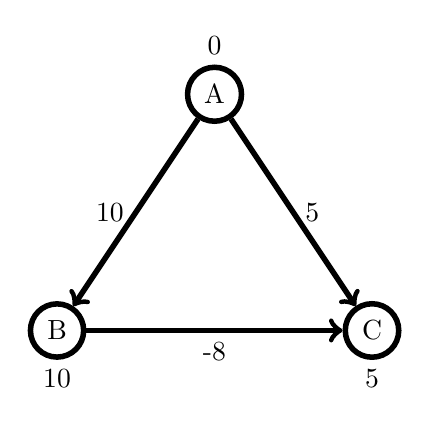
\begin{tikzpicture}
            % Nodes
            \node[circle, draw, line width=2pt] (A) at (0, 0) {A};
            \node[circle, draw, line width=2pt] (B) at (-2, -3) {B};
            \node[circle, draw, line width=2pt] (C) at (2, -3) {C};

            % Additional labels
            \node[above] at (A.north) {0};
            \node[below] at (B.south) {10};
            \node[below] at (C.south) {5};

            % Edges
            \draw[->, line width=2pt] (A) -- (B) node[midway, left] {10};
            \draw[->, line width=2pt] (A) -- (C) node[midway, right] {5};
            \draw[->, line width=2pt] (B) -- (C) node[midway, below] {-8};
        \end{tikzpicture}
        \caption{First iteration of Dijkstra's algorithm.}
        \label{fig:Dijkstra}
    \end{figure}

    \clearpage

    \question[15] [W6, \stars{3}] Assume Bellman-Ford has identified the presence of a negative-weight cycle (in the second for loop in the algorithm in the slides). Explain how to identify and output the vertices that constitute this cycle.

    This can be done simply by traverseing through the predecessor array.

    \begin{minted}{python}
        def find_negative_cycle(pred, start):
            cycle = []
            current = start
            while True:
                cycle.append(current)
                current = pred[current]
                if current == start:
                    break
            return cycle
    \end{minted}

    Where \texttt{pred} is the predecessor array and \texttt{start} is the vertex that is the start of the cycle. This function will return a list of vertices that constitute the negative-weight cycle.

    \clearpage
    \question[10] [W7, \stars{1}] For the following questions, select the true statement(s). \textbf{No explanation is necessary for these questions.}

    \begin{parts}
        \part What is true about the residual graph in the Ford-Fulkerson algorithm?

        $\blacksquare$ The sum of residual capacities over all edges in the residual graph is equal to the sum of the capacities in the original graph. \\
        $\square$ The number of edges in the residual graph is at least equal to the number of directed edges in the flow network. \\
        $\blacksquare$ The capacity of any edge in residual graph does not exceed the capacity of the corresponding edge in the flow network, if it exists. \\
        $\square$ The capacity of an edge in the residual graph depends on the direction, quantity, and capacities of the pipes between the two vertices.

        \part What must be true if there is a directed path in the residual graph from the source to the sink in the Ford-Fulkerson algorithm?

        $\square$ The flow is not maximized. \\
        $\blacksquare$ The path is an augmenting path. \\
        $\square$ There is a cut in the original flow graph whose capacity is equal to the flow in the network.
    \end{parts}
    \clearpage

    \question[10] [W7, \stars{1}] Flow. For the following questions, select whether the statement is true or false,
    and write a \textit{brief} explanation of your reasoning.
    \begin{parts}
        \part The maximum flow in a flow network is equal to the minimum cut of the network.\\
        $\square$ True $\blacksquare$ False

        This is false because the maximum flow in a flow network is the maximum amount of flow that can be pushed through the network. The minimum cut of the network is the minimum capacity of the edges that need to be removed to disconnect the source from the sink. These two values are not necessarily equal.

        \textit{Max flow is equal to the minimum cut if and only if the flow is maximized and the residual graph has no augmenting paths from the source to the sink.}

        \part In the residual graph of the maximum flow, there are no augmenting paths from the source to the sink. \\
        $\blacksquare$ True $\square$ False

        This is true because if there are no augmenting paths from the source to the sink, then the flow is maximized. (ie there is no more flow that can be pushed through the network.)

        \part In a residual network, the capacity of an edge can be zero.\\
        $\blacksquare$ True $\square$ False

        This is true because when the capacity of an edge is zero in a residual network, it means that the edge is saturated and no flow can pass through it. (The edge is effectively removed from the residual.)

        \part If a single edge's capacity in a flow network is increased, the maximum flow value can only either stay the same or increase.\\
        $\blacksquare$ True $\square$ False

        This is true because the maximum flow value is the maximum amount of flow that can be pushed through the network. You can't decrease the max flow by making an edge more capable of carrying flow.

    \end{parts}
    \clearpage
    \question[20] [W7, \stars{3}] How can standard, unmodified max-flow algorithms (which only work with a single source and single sink node) be applied to a graph with multiple sources and sinks? Describe the necessary steps or considerations.

    To run unmodified max-flow algorithms, like Ford-Fulkerson, on a graph with multiple sources and sinks, we can create a new master source and sink node and connect the original sources and sinks to the new master source and sink. The capacity of these edges will infinity or at least greater than or equal to the total capacity of the original source/sink it connects. This will create a single source and single sink graph that can be used with the unmodified max-flow algorithm.

    \clearpage

    % close the document
\end{questions}
\end{document}
